% CS-781 Capstone report — Rohit Batra (261110054).
% Self-contained layout (two-column, 10pt). If the course template is used, copy the body (from \begin{abstract} on)
% into it; figures come from report/figures/ and tables from report/tables/ (both rebuilt by report/make_*.py).
\documentclass[10pt,twocolumn]{article}
\usepackage[a4paper,margin=0.72in,columnsep=0.25in]{geometry}
\usepackage[T1]{fontenc}
\usepackage{times}
\usepackage{microtype}
\usepackage{graphicx}
\usepackage{booktabs}
\usepackage{tabularx}
\usepackage{longtable}
\usepackage{amsmath}
\usepackage{xcolor}
\usepackage[hidelinks]{hyperref}
\usepackage{enumitem}
\setlist{nosep,leftmargin=*}
\graphicspath{{figures/}}
\newcommand{\A}{\textsf{A}}\newcommand{\B}{\textsf{B}}\newcommand{\C}{\textsf{C}}\newcommand{\D}{\textsf{D}}

\title{\vspace{-1.2em}A Self-Hosted Legal Language Model: Four From-Scratch Architectures\\
Adapted to Six Indian Legal NLP Tasks\vspace{-0.3em}}
\author{Rohit Batra \quad Roll No.\ 261110054 \quad Codabench: \texttt{r\_261110054}\\
CS-781 Capstone, IIT Kanpur\\ \small\url{https://github.com/Rohit2004Batra/cs781-legal-lm-capstone}}
\date{\vspace{-1.5em}}

\begin{document}
\maketitle

\begin{abstract}
We train four compact language models from scratch (103--139M parameters) on the official Indian legal corpus: a decoder-only Transformer (\A), an encoder--decoder Transformer (\B), a stacked LSTM (\C) and a dilated residual TCN (\D). We adapt them, without any external weights, to named-entity recognition, rhetorical roles, judgment prediction, statute identification, summarisation and prior-case retrieval.
Across 38 submissions we compare full, layer-wise and bias-only fine-tuning; LoRA, LORMA, IA$^3$, prefix and prompt tuning; adapters; and knowledge distillation (KD).
\begin{itemize}
\item \textbf{Best results:} 0.806 BERTScore (pretraining), 0.491 strict Macro-F1 (NER), 0.518 Macro-F1 (rhetorical roles), 0.680 Macro-F1 (judgment), 0.304 Macro-F1 (statutes), 0.835 BERTScore (summaries) and 0.253 Micro-F1@7 (retrieval).
\item \textbf{The backbone mattered:} the decoder \A{} transferred best to every task except character-level NER.
\item \textbf{Three methods mattered most:} a linear-probe-then-fine-tune schedule (LP-FT), which ended a series of training collapses; per-label decision calibration; and distillation, which twice produced a smaller student that beat its own teacher.
\end{itemize}
\end{abstract}

\section{Introduction}
A law firm that cannot send client documents to an outside API needs a model it can host itself.
The capstone builds such a model in two stages:
\begin{itemize}
\item \textbf{Phase~1:} pretrain small language models from scratch on legal text.
\item \textbf{Phases 2--7:} adapt them to downstream tasks under fixed rules: every experiment starts from the Phase-1 weights, LORMA \cite{lorma} is compulsory, and at least one KD run is required per phase.
\end{itemize}
Compute was limited to free Kaggle T4 GPUs.

\textbf{Contributions.}
\begin{enumerate}
\item Four architecturally different legal LMs and one shared 50K byte-level BPE tokenizer (\S\ref{sec:p1}).
\item One adaptation framework reused across all phases (\S\ref{sec:methods}): Phase-1 backbone $\rightarrow$ PEFT method $\rightarrow$ task head, with chunked long documents, standardised features and LP-FT \cite{lpft}.
\item Controlled comparisons of nine adaptation techniques and the four backbones on six tasks (\S\ref{sec:exp}), with data-driven design choices (\S\ref{sec:data}) and validation estimates that tracked the hidden test scores (Fig.~\ref{fig:valtest}).
\item An account of what failed and why (\S\ref{sec:failed}), including a four-run collapse of LORMA and its diagnosis.
\end{enumerate}
Every notebook, phase README, design decision and score is in the GitHub repository above. Appendix~\ref{app:subs} lists all 38 submissions.

\section{Data and what it implied}\label{sec:data}
Each phase began with a data-analysis notebook; its outputs are in the repository. Table~\ref{tab:data} summarises the task data and the finding that shaped each design.

\begin{table}[t]\centering\footnotesize\setlength{\tabcolsep}{3pt}
\begin{tabularx}{\columnwidth}{@{}l p{2.3cm} X@{}}\toprule
Ph. & Data (train / dev / test) & Key finding $\rightarrow$ design \\\midrule
1 & 4.34B tok.\ (4 sources) & 91\% from high courts and tribunals $\rightarrow$ 25\% equal mix \\
2 & 70 / -- / 35 docs, 8.4k spans & 96\% of gold starts fall inside a BPE token $\rightarrow$ character-level boundaries \\
3 & 80 / 10 / 10 docs, 17k sents & context matters; 0.05--28\% label skew $\rightarrow$ sentence encoder + document BiLSTM-CRF \\
4 & 31.6k / 1,988 / 1,517 & \textbf{test $\subset$ dev} $\rightarrow$ ``dev-clean''; outcome cues at the end $\rightarrow$ last chunks \\
5 & 42.8k / 10.2k / 13.0k, 100 labels & 42\% of dev label sets unseen $\rightarrow$ binary relevance + per-statute thresholds \\
6 & 7,030 / -- / 100 & content spread evenly over the case $\rightarrow$ chunk-level summaries \\
7 & 827 / 118 / 237 queries & every query is in its own pool; BM25 on the full text is weak $\rightarrow$ exclude self; first and last chunks \\\bottomrule
\end{tabularx}
\caption{Task data and the decision each analysis led to.}\label{tab:data}\vspace{-1em}
\end{table}

Two findings protected the scores from leakage or a trivial loss:
\begin{itemize}
\item In Phase~4, all 1,517 test cases also appear in dev \emph{with labels}. We never trained or tuned on them: selection used the 1,988 remaining dev cases.
\item In Phase~7, every query sits in its own candidate pool. Without exclusion, the query itself would be every query's first answer.
\end{itemize}

Other choices that followed from the analysis:
\begin{itemize}
\item \textbf{Casing:} train and test casing differed in Phase~4, and the tokenizer is cased, so we lower-cased there and nowhere else.
\item \textbf{Placeholders:} masked placeholders (\texttt{<SECTION>}, \texttt{<CITATION>}, \texttt{<ORG>}) were mapped to plain words; they cost 3--5 BPE tokens each.
\end{itemize}

\section{Foundation models (Phase 1)}\label{sec:p1}
\textbf{Tokenizer.} Our own byte-level BPE (vocabulary 50,000, trained on 25M characters per source); a GPT-2 tokenizer would have been trained on web text.

\textbf{Training.}
\begin{itemize}
\item Every model saw \textbf{100M tokens}, sampled equally from acts, high courts, the Supreme Court and tribunals.
\item AdamW, learning rate $3\!\times\!10^{-4}$ with cosine decay, 16k tokens per step, one T4, bf16.
\item Checkpoint selection on a 2\% hash-split held-out set.
\end{itemize}

\begin{table}[t]\centering\footnotesize\setlength{\tabcolsep}{3pt}
\begin{tabular}{@{}l l r r r r@{}}\toprule
 & Architecture & Params & Ctx & PPL & BERTSc. \\\midrule
\A & decoder, 12L, $d$=768 & 125.0M & 2048 & \textbf{20.3} & 0.793 \\
\B & enc--dec, 6+6L & 139.3M & 1k+1k & 31.8 & \textbf{0.806} \\
\C & LSTM, 3$\times$1280 & 103.4M & 1024 & 48.0 & 0.802 \\
\D & TCN, 10 blocks & 114.2M & 2048 & 48.2 & 0.805 \\\bottomrule
\end{tabular}
\caption{Phase-1 models. PPL: held-out next-token perplexity. BERTScore F1: Codabench, 128-word continuations of 512-word prompts.}\label{tab:p1}\vspace{-1em}
\end{table}

\textbf{Results (Table~\ref{tab:p1}).}
\begin{itemize}
\item \A{} has by far the lowest perplexity but the lowest BERTScore.
\item The four models were decoded differently: \A{} and \C{} with near-greedy sampling (temperature 0.1), \B{} and \D{} at 0.7--0.8. Near-greedy decoding favours repetition.
\item BERTScore is also compressed: all four scores lie within 0.013.
\item Perplexity turned out to be the better predictor of downstream value: \A{} became the strongest backbone in Phases 3--7.
\end{itemize}

\section{Adaptation framework}\label{sec:methods}
Every submission is \emph{Phase-1 backbone + adaptation technique + task head}. Each notebook is self-contained and resumes from checkpoints.

\textbf{Techniques.}
\begin{itemize}
\item Full, layer-wise and bias-only (BitFit \cite{bitfit}) fine-tuning.
\item LoRA \cite{lora}.
\item \textbf{LORMA} \cite{lorma}: a multiplicative low-rank update $W_{\text{eff}}=(I+\tfrac{\alpha}{r}BA)W_0$ with $B\!=\!0$ at the start. We used $r\!=\!8$ and $\alpha\!=\!16$ on q, k, v, out, fc1 and fc2 of \A{}, and on the recurrent gates of \C{}.
\item IA$^3$ \cite{ia3}, prefix \cite{prefix} and prompt tuning \cite{prompt}, and Houlsby / bottleneck adapters \cite{houlsby}.
\item KD \cite{hinton}.
\end{itemize}

\textbf{Long documents.}
\begin{itemize}
\item Cases are split into 510-token chunks. A chunk becomes [mean; final state] of its token states.
\item Chunks are pooled per case with attention, mean or max. Positional chunk selection (first or last chunks) follows each task's data analysis.
\end{itemize}

\textbf{Feature standardisation.} \A's residual stream has a few nearly constant dimensions ($|x|\!\approx\!46$ against a mean of 2) that swamp any normalisation. We therefore standardise token or chunk features per dimension, using statistics from the frozen model. Phase~4 showed this matters (\S\ref{sec:failed}).

\textbf{LP-FT \cite{lpft}.}
\begin{itemize}
\item First a linear probe (or a retrieval projection) is trained on cached frozen features and copied into the model as ``epoch~0''.
\item Then the adapter and head are fine-tuned gently.
\item The best of epochs $0,\dots,E$ on validation is kept, so a run can never end below its probe.
\end{itemize}

\textbf{KD.} Students are smaller Phase-1 models, e.g.\ every other layer of \A{} (as in DistilBERT \cite{distilbert}). They learn from the teacher's soft labels, logits or similarity distributions (temperature 2) plus the gold loss.

\section{Experiments}\label{sec:exp}
Table~\ref{tab:main} lists the submissions counted in each phase. Appendix~\ref{app:subs} lists every run, and Appendix~\ref{app:hp} the settings.

\begin{table*}[t]\centering\footnotesize\setlength{\tabcolsep}{4pt}
\begin{tabularx}{\textwidth}{@{}l l X r r r@{}}\toprule
Phase (metric) & Sub. & Backbone + technique (head / key choice) & Trainable & Validation & \textbf{Test} \\\midrule
2 NER & S1 & \A{} full fine-tuning (char-level start/end head) & 125.6M & 0.225 & 0.192 \\
(strict Macro-F1) & S2 & \B{} encoder + LoRA (QKV, then +out/FFN) & 0.91M & 0.198 & 0.177 \\
 & S3 & \C{} + \textbf{LORMA} on recurrent weights; span caps + per-label thresholds & 0.79M & 0.494 & \textbf{0.491} \\
 & S4 & KD: \D{} teacher (4 blocks tuned) $\rightarrow$ 6-block \D{} student & 38.4M & 0.220 & 0.253 \\\midrule
3 Rhetorical roles & S1 & \C{} + \textbf{LORMA} + document BiLSTM & 3.39M & $\approx$0.40 & 0.402 \\
(Macro-F1) & S3 & \B{} encoder + IA$^3$ + document BiLSTM & 2.40M & 0.219 & 0.236 \\
 & S4 & \D{} + prompt tuning (20 tokens) + document BiLSTM & 2.66M & 0.329 & 0.339 \\
 & S7 & \A{} + LoRA (attn+FFN) + BiLSTM-CRF; stage 2 on train+dev & 3.70M & 0.450 & 0.502 \\
 & S6 & KD: S7 $\rightarrow$ 6-layer \A{} student (66\% of params) & 3.04M & 0.458 & \textbf{0.518} \\\midrule
4 Judgment & S1 & \A{} + \textbf{LORMA}, LP-FT, last 2 chunks & 1.33M+head & 0.695 & \textbf{0.680} \\
(Macro-F1) & S2 & \C{} layer-wise FT (top LSTM layer) & 13M & 0.562 & 0.562 \\
 & S3 & \B{} encoder + BitFit & --- & 0.531 & 0.491 \\
 & S4 & \D{} + bottleneck adapters & --- & 0.578 & 0.527 \\
 & S5 & KD: S2 $\rightarrow$ 2-layer \C{} student & --- & 0.613 & 0.592 \\\midrule
5 Statutes & S1 & \A{} + \textbf{LORMA}, LP-FT, per-statute thresholds & 1.63M & 0.298 & \textbf{0.304} \\
(Macro-F1) & S2 & \C{} layer-wise FT & 13.6M & 0.273 & 0.263 \\
 & S3 & \D{} + bottleneck adapters & 1.73M & 0.271 & 0.273 \\
 & S4 & KD: S1+S2+S3 ensemble $\rightarrow$ \B{} encoder + LoRA & 0.90M & 0.215 & 0.220 \\\midrule
6 Summaries & S1 & \A{} + \textbf{LORMA} prefix-LM, chunk summaries; tuned decoding & --- & R1 0.521 & \textbf{0.835} \\
(BERTScore F1) & S2 & \B{} + LoRA on all projections; tuned decoding & --- & --- & 0.809 \\
 & S3 & \D{} + Houlsby adapters; tuned decoding & --- & --- & 0.814 \\
 & S4 & KD: S1 $\rightarrow$ \C{} (word-level KL); tuned decoding & --- & --- & 0.816 \\\midrule
7 Retrieval & S1 & \A{} + \textbf{LORMA} bi-encoder, InfoNCE + TF-IDF hard negatives & 1.72M & 0.269 & \textbf{0.253} \\
(Micro-F1@7) & S2 & \C{} layer-wise FT bi-encoder & 13.8M & 0.217 & 0.180 \\
 & S3 & \D{} + prompt tuning bi-encoder & 0.55M & 0.198 & 0.181 \\
 & S4 & KD: S1 $\rightarrow$ 6-layer \A{} (listwise KL + teacher negatives) & 1.06M & 0.280 & 0.237 \\\bottomrule
\end{tabularx}
\caption{Counted submissions per phase. Validation scores never use test labels: Phase~4 uses dev-clean, Phase~5 cross-fitted thresholds, and Phase~3 the 13-label average. ``---'': not recorded. The best result per phase is in bold.}\label{tab:main}\vspace{-0.8em}
\end{table*}

\textbf{Phase 2 (NER).}
\begin{itemize}
\item Byte-level BPE attaches the leading space to the following token (\texttt{\.GCOURT}), so 97\% of gold starts sit one character inside a token. We therefore predict start and end per \emph{character}: each character gets its token's state plus a character embedding. Decoding with perfect boundary probabilities reproduces 100\% of the spans.
\item \C{}+LORMA won by a wide margin.
\item Calibrating span-length caps and thresholds per label added +0.10 (0.392$\rightarrow$0.494).
\item Full fine-tuning of \A{} had not converged after 903 steps at learning rate $10^{-5}$.
\end{itemize}

\textbf{Phase 3 (rhetorical roles).}
\begin{itemize}
\item \textbf{Context:} a document BiLSTM over sentence vectors roughly doubles Macro-F1 over sentence-only probes (\A: 0.283$\rightarrow$0.440; Fig.~\ref{fig:context}). A CRF adds another +0.02 to +0.04.
\item \textbf{LoRA beat prefix tuning} in an otherwise identical pipeline (0.502 vs 0.453).
\item \textbf{IA$^3$ underfitted} the weakest backbone.
\item \textbf{The KD student beat its teacher} (0.518 vs 0.502) with 66\% of the parameters, 1.5$\times$ faster and at half the GPU memory.
\end{itemize}

\textbf{Phase 4 (judgment prediction).}
\begin{itemize}
\item The last two chunks carry the outcome signal: first two chunks 0.593 vs last two 0.695.
\item \A{}+LORMA collapsed to a constant prediction four times. LP-FT fixed it: the probe alone gave 0.606, and LORMA fine-tuning added +0.088 (\S\ref{sec:failed}).
\item The distilled two-layer LSTM again beat its teacher (0.592 vs 0.562).
\end{itemize}

\textbf{Phase 5 (statutes).}
\begin{itemize}
\item Per-statute thresholds were tuned with cross-fitting, i.e.\ tuned on one half of dev and scored on the other. Thresholds tuned and scored on the same dev data overstate Macro-F1 by about 0.015.
\item The cross-fitted estimates landed within $\pm$0.01 of test for all four runs.
\item Per-statute F1 rises with training frequency (quartile 1 0.20 $\rightarrow$ quartile 4 0.45).
\item The typical error is a specific statute replaced by a frequent, generic one.
\end{itemize}

\textbf{Phase 6 (summarisation).}
\begin{itemize}
\item Summarising every chunk and joining the results beats summarising the first chunk alone by +0.16 ROUGE-1.
\item Changing only the decoding (minimum length 22\% of the chunk plus a CTRL repetition penalty \cite{ctrl} of 1.2) raised BERTScore by +0.006 to +0.008 and ROUGE-1 by +0.04 to +0.08 for \emph{every} model, without retraining (Fig.~\ref{fig:dec}). Repeated trigrams fell from 20\% to 11\%.
\item The \C{} student distilled from \A{} beat the directly adapted \B{} and \D{}.
\end{itemize}

\textbf{Phase 7 (prior-case retrieval).}
\begin{itemize}
\item \textbf{Model:} a bi-encoder. Each case vector is the normalised mean of chunk vectors over the first 8 and last 8 chunks; relevance is cosine similarity.
\item \textbf{Training:} InfoNCE (temperature 0.05) with TF-IDF hard negatives and in-batch negatives, and LP-FT.
\item \textbf{Transfer:} frozen Phase-1 vectors already retrieve (\A{} 0.238 on dev). The contrastive projection gives most of the gain.
\item \textbf{KD:} the 6-layer student encodes 1.99$\times$ faster with 66\% of the parameters and keeps 94\% of the teacher's test score.
\item \textbf{Ceiling and reference:} with exactly 7 answers per query, an oracle reaches only 0.62 on dev. All four models stay below the TF-IDF reference (0.368 dev), but their hits are partly different from TF-IDF's: 393 relevant cases found by either vs 331 by TF-IDF alone.
\end{itemize}

\begin{figure*}[t]\centering
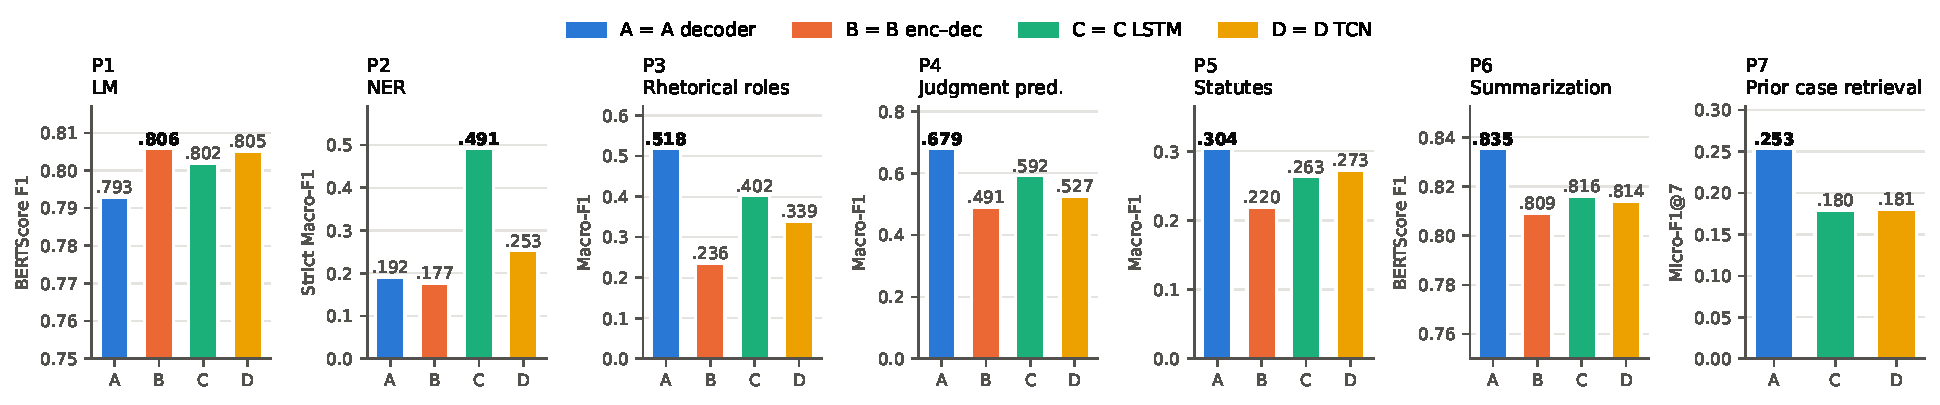
\includegraphics[width=\textwidth]{fig1_scores_by_phase_and_backbone.pdf}\vspace{-0.6em}
\caption{Best test score per backbone and phase. \A{} wins every downstream phase except NER (\C).}\label{fig:backbones}\vspace{-0.6em}
\end{figure*}

\begin{table}[t]\centering\footnotesize\setlength{\tabcolsep}{3pt}
\begin{tabularx}{\columnwidth}{@{}l X r@{}}\toprule
Ph. & Controlled change (everything else fixed) & $\Delta$ (val.) \\\midrule
2 & per-label span caps + thresholds (S3) & +0.102 \\
3 & + document BiLSTM vs sentence-only (\A{}, S2) & +0.158 \\
3 & Viterbi CRF vs argmax (S7) & +0.042 \\
3 & prefix tuning vs LoRA, same pipeline (test) & $-$0.049 \\
4 & last 2 vs first 2 chunks (S1) & +0.102 \\
4 & LORMA fine-tuning over its linear probe (S1) & +0.088 \\
5 & first chunk only vs evidence chunks (S1) & $-$0.035 \\
5 & thresholds scored on their own tuning data & +0.015$^\dagger$ \\
6 & all chunks joined vs first chunk (ROUGE-1, S1) & +0.158 \\
6 & tuned decoding, same weights (ROUGE-1, S1) & +0.060 \\
7 & contrastive projection on frozen \C{} features & +0.074 \\
7 & mean vs max pooling over chunks (S1) & +0.089 \\
7 & first 8 + last 8 vs first chunk only (S1) & +0.157 \\\bottomrule
\end{tabularx}
\caption{Controlled ablations (validation; Phase~6 in ROUGE-1). $^\dagger$An optimistic bias, which is why Phase~5 reports cross-fitted estimates.}\label{tab:abl}\vspace{-1em}
\end{table}

\section{Cross-phase analysis}\label{sec:analysis}
\textbf{What moved the scores (Table~\ref{tab:abl}).} The largest controlled gains came from task structure rather than from the adapter itself: which part of the document is read, document-level context, and calibrating decisions or decoding. Within a fixed backbone, the adapter changed scores by 0.02--0.09.
\textbf{Which backbone transfers (Fig.~\ref{fig:backbones}).}
\begin{itemize}
\item The decoder \A{} is best in Phases 3--7, and frozen-feature probes predict this ranking before any training.
\item \C{} wins only NER, where boundaries are local and recurrence suits character-level decisions.
\item The encoder of \B{} was consistently weakest when frozen. Its decoder was trained to read it, not to be a feature extractor.
\end{itemize}

\textbf{PEFT vs full adaptation.} On small datasets (70 NER documents, 80 rhetorical-role documents, 817 retrieval queries), PEFT beat or matched heavier tuning:
\begin{itemize}
\item full fine-tuning of 125M parameters lost to LORMA on 0.8M (NER);
\item layer-wise tuning of 13M parameters tied prompt tuning on 0.55M (retrieval).
\end{itemize}
Capacity still has a floor: IA$^3$ (27.6K parameters) and BitFit underfitted. Techniques that \emph{add new directions} to the weights (LoRA, LORMA) beat those that only rescale (IA$^3$, BitFit) or only add inputs (prefix, prompt).

\textbf{Does KD preserve quality?} Yes, in all six phases. Students beat their teachers twice (rhetorical roles, judgment) and kept 94\% in retrieval. In a fourth phase the distilled LSTM beat two directly adapted models (summaries). Students lost when they came from a weak backbone: the \B{} encoder kept 69\% in Phase~5. KD worked as a regulariser on small, noisy data as much as as compression.

\textbf{Were the validation estimates reliable? (Fig.~\ref{fig:valtest}).} Leak-free validation ranked submissions as the test did in every phase. The largest gaps came from the smallest dev sets (10 documents in Phase~3, 118 queries in Phase~7).

\begin{figure*}[t]\centering
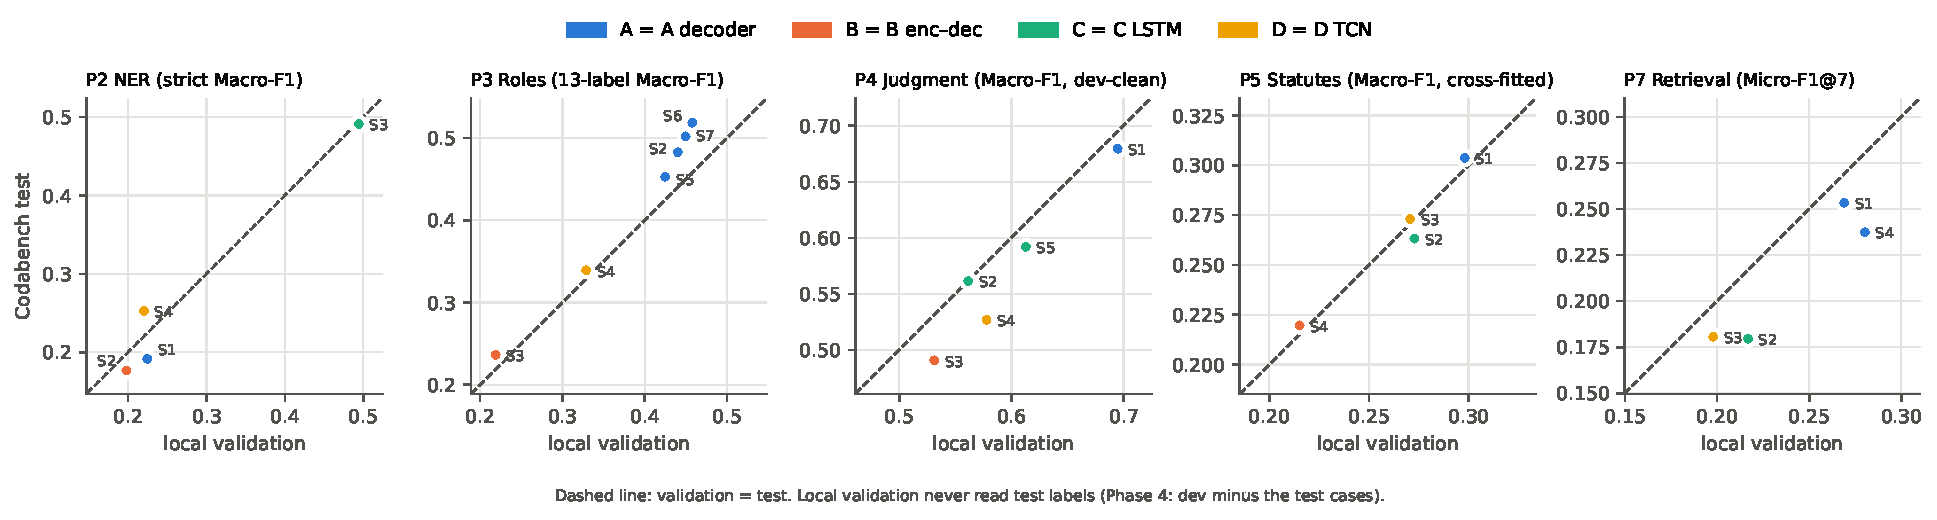
\includegraphics[width=\textwidth]{fig2_validation_vs_codabench.pdf}\vspace{-0.6em}
\caption{Local validation vs Codabench test, for every submission with a comparable validation score.}\label{fig:valtest}\vspace{-0.8em}
\end{figure*}

\textbf{Cost vs score.} The best runs were not the most expensive per point:
\begin{itemize}
\item LORMA on \A{} trained only 1.3--1.7M parameters, at 2--9~GB of GPU memory and 45--160 minutes per run.
\item Decoding changes in Phase~6 cost no training at all.
\end{itemize}

\section{What failed and why}\label{sec:failed}
\textbf{LORMA collapse (Phase 4).} \A{}+LORMA predicted one class for every case in four consecutive runs. We changed one suspected cause at a time:
\begin{enumerate}
\item Attention pooling: no effect.
\item Standardising token states: the diagnostic notebook found nearly constant outlier dimensions. Still collapsed.
\item Turning off dropout in the frozen backbone: dropping one outlier dimension shifts LayerNorm for the whole token. Still collapsed.
\end{enumerate}
\textbf{Final cause:} with a randomly initialised head, the first multiplicative updates wreck the features before the head finds the weak signal. LP-FT solved it, and the same schedule then worked in Phases 5 and 7.

\textbf{Other failures.}
\begin{itemize}
\item \textbf{Phase 1 decoding:} near-greedy sampling for \A{} and \C{} (repetition).
\item \textbf{Phase 2:} full fine-tuning of \A{} at a learning rate that was too low; a ``LORMA'' that was in fact additive, replaced by the true multiplicative form.
\item \textbf{Phase 3:} the TCN's dilated convolutions hit a slow GPU path (220 minutes per epoch); rewriting them as exact per-tap matrix multiplies made them about 120$\times$ faster.
\item \textbf{Phase 6:} the original decoding was too short and repetitive.
\item \textbf{Phase 7:} the neural rankers stayed below TF-IDF. A next-token objective over 100M tokens does not encode \emph{which legal issue} a case is about, and 817 queries with roughly 15 in-batch negatives cannot reshape that much.
\end{itemize}

\section{Limitations and future work}
\textbf{Limitations.}
\begin{itemize}
\item Each Phase-1 model saw only 2.3\% of the corpus (100M of 4.3B tokens); all were still improving except \A.
\item Most runs were limited to 2--4 epochs by Kaggle session limits.
\item Several validation sets were tiny (10 documents, 118 queries).
\item Peak-memory figures are missing for Phases 1 and 4, and the Phase-7 KD memory comparison did not separate the two models.
\end{itemize}

\textbf{Future work.}
\begin{itemize}
\item Pretrain longer with a retrieval-aware objective (contrastive pairs from citations).
\item Use larger in-batch negative pools via gradient caching.
\item Combine neural and lexical scores in Phase~7, which the complementary hits suggest.
\item Use a single \A-family student, distilled once, for all tasks.
\end{itemize}

\section{Conclusion}
A self-hosted 125M-parameter decoder trained on 100M legal tokens, adapted with about 1\% extra parameters through LORMA and LP-FT, reached the best result in five of six downstream tasks. Distilled students of 66\% size kept, and twice exceeded, their teachers' quality.
The largest gains came less from the choice of adapter than from:
\begin{itemize}
\item reading the data correctly (leaks, token boundaries, which part of a document matters);
\item stable optimisation (standardisation, LP-FT);
\item calibrating decisions (thresholds, decoding).
\end{itemize}

\section*{LLM usage declaration}
\textcolor{red}{[Replace with the questionnaire from the official template.]}
\begin{itemize}
\item \textbf{Tool:} Claude (Anthropic) was used as a coding and writing assistant.
\item \textbf{What it did:} drafting the Kaggle notebooks from our specifications, debugging (e.g.\ the Phase-4 collapse diagnosis), writing the READMEs, and drafting this report.
\item \textbf{What it did not do:} it used no project data and produced no model outputs. No LLM or API was used inside any submitted model, and no pretrained weights were used.
\item \textbf{What we did:} all notebooks were run, checked and submitted by the author, and all numbers come from our own runs.
\end{itemize}

{\footnotesize
\begin{thebibliography}{99}\setlength{\itemsep}{0pt}
\bibitem{lorma} H.~Bihany, S.~Patel, A.~Modi. LoRMA: Low-Rank Multiplicative Adaptation for LLMs. \emph{Findings of ACL}, 2025.
\bibitem{lora} E.~Hu et al. LoRA: Low-Rank Adaptation of Large Language Models. \emph{ICLR}, 2022.
\bibitem{lpft} A.~Kumar et al. Fine-Tuning can Distort Pretrained Features and Underperform Out-of-Distribution. \emph{ICLR}, 2022.
\bibitem{ia3} H.~Liu et al. Few-Shot Parameter-Efficient Fine-Tuning is Better and Cheaper than In-Context Learning. \emph{NeurIPS}, 2022.
\bibitem{prefix} X.~L.~Li, P.~Liang. Prefix-Tuning. \emph{ACL}, 2021.
\bibitem{prompt} B.~Lester, R.~Al-Rfou, N.~Constant. The Power of Scale for Parameter-Efficient Prompt Tuning. \emph{EMNLP}, 2021.
\bibitem{houlsby} N.~Houlsby et al. Parameter-Efficient Transfer Learning for NLP. \emph{ICML}, 2019.
\bibitem{bitfit} E.~Ben Zaken, S.~Ravfogel, Y.~Goldberg. BitFit. \emph{ACL}, 2022.
\bibitem{hinton} G.~Hinton, O.~Vinyals, J.~Dean. Distilling the Knowledge in a Neural Network. \emph{arXiv:1503.02531}, 2015.
\bibitem{distilbert} V.~Sanh et al. DistilBERT. \emph{arXiv:1910.01108}, 2019.
\bibitem{ctrl} N.~S.~Keskar et al. CTRL: A Conditional Transformer Language Model. \emph{arXiv:1909.05858}, 2019.
\bibitem{infonce} A.~van den Oord, Y.~Li, O.~Vinyals. Representation Learning with Contrastive Predictive Coding. \emph{arXiv:1807.03748}, 2018.
\bibitem{tcn} S.~Bai, J.~Z.~Kolter, V.~Koltun. An Empirical Evaluation of Generic Convolutional and Recurrent Networks. \emph{arXiv:1803.01271}, 2018.
\bibitem{crf} J.~Lafferty, A.~McCallum, F.~Pereira. Conditional Random Fields. \emph{ICML}, 2001.
\bibitem{bm25} S.~Robertson, H.~Zaragoza. The Probabilistic Relevance Framework: BM25 and Beyond. \emph{FnTIR}, 2009.
\end{thebibliography}}

\onecolumn
\appendix
\section{All submissions}\label{app:subs}
Every Codabench run, from \texttt{results/submissions.csv}. The \emph{Kept} column marks the runs on the final leaderboard. Replaced runs: Phase~3 S2 and S5 (now ablations: LoRA without a CRF; prefix tuning vs LoRA), the two earlier Phase-4 S1 runs (superseded by the final LP-FT run), and the original Phase-6 decoding (superseded by the tuned decoding of the same weights).
{\scriptsize\begin{longtable}{@{}l p{4.1cm} p{5.2cm} r p{3.0cm} r l@{}}
\toprule Ph. & Notebook & Base model / technique & Trainable & Local validation & Test & Kept \\ \midrule \endhead
\bottomrule \endfoot
1 & A\_decoder\_only & A Decoder-only: from-scratch pretraining & 125.03M & val PPL 20.30 & 0.7929 & yes \\
1 & B\_Encoder\_Decoder & B Encoder-Decoder: from-scratch pretraining & 139.26M & val PPL 31.82 & 0.8058 & yes \\
1 & C\_StackedLSTM & C Stacked LSTM: from-scratch pretraining & 103.40M & val PPL 47.97 & 0.8020 & yes \\
1 & D\_TCN & D TCN: from-scratch pretraining & 114.16M & val PPL 48.17 & 0.8052 & yes \\
2 & S1\_Decoder\_FullFineTuning & A Decoder-only: full fine-tuning & 125.64M & 0.2245 & 0.1916 & yes \\
2 & S2\_Encoder\_Decoder\_LORA & B Encoder-Decoder: LoRA / expanded LoRA & 0.91M & 0.1976 & 0.1768 & yes \\
2 & S3\_StackedLSTM\_LORAM & C Stacked LSTM: LORMA & 0.79M & 0.4943 & 0.4912 & yes \\
2 & S4\_TCN\_KnowDist & D TCN: knowledge distillation & 38.45M & 0.2202 & 0.2527 & yes \\
3 & P3\_S1\_C\_LSTM\_LORMA & C Stacked LSTM: LORMA r=8 + doc BiLSTM & 3.39M & 0.4762 (dev; CL 0.3902 IT 0.4695) & 0.4024 & yes \\
3 & P3\_S2\_A\_Decoder\_LoRA & A Decoder-only: LoRA r=8 q/k/v/out + doc BiLSTM & 2.96M & 0.4402 (dev 13-label; present 0.5202) & 0.4825 & no \\
3 & P3\_S3\_B\_Encoder\_IA3 & B Encoder-Decoder (encoder): IA3 keys/values/FFN + doc BiLSTM & 2.40M & 0.2188 (dev 13-label; present 0.2586) & 0.2364 & yes \\
3 & P3\_S4\_D\_TCN\_PromptTuning & D Dilated Residual TCN: Prompt tuning 20 tokens + doc BiLSTM & 2.66M & 0.3289 (dev 13-label; present 0.3886) & 0.3391 & yes \\
3 & P3\_S7\_A\_LoRA\_CRF\_TrainDev & A Decoder-only: LoRA attn+FFN + BiLSTM-CRF; Stage 2 train+dev & 3.70M & 0.4497 (Stage-1 dev 13-label Viterbi; argmax 0.4082) & 0.5019 & yes \\
3 & P3\_S5\_A\_Prefix\_CRF\_TrainDev & A Decoder-only: Prefix tuning 20x12 (MLP) + BiLSTM-CRF; Stage 2 train+dev & 12.24M & 0.4249 (Stage-1 dev 13-label Viterbi; argmax 0.4063) & 0.4527 & no \\
3 & P3\_S6\_KD\_S7Teacher\_6LayerStudent & A 6 of 12 layers (student): KD from S7 (T=2) + LoRA + BiLSTM-CRF; Stage 2 train+dev & 3.04M & 0.4579 (student Stage-1 dev; teacher 0.4497) & 0.5184 & yes \\
4 & P4\_S1\_A\_LORMA & A Decoder-only: LORMA r=8 attn+FFN; last 2x510 chunks; standardised states & -- & 0.3452 (dev-clean; collapsed) & 0.3475 & no \\
4 & P4\_S2\_C\_LSTM\_LayerwiseFT & C Stacked LSTM: Layer-wise FT: top LSTM layer + final norm; last 4 chunks at test & -- & 0.5615 (dev-clean last 4) & 0.5615 & yes \\
4 & P4\_S3\_B\_Encoder\_BitFit & B Encoder (6L): BitFit bias-only & -- & 0.5312 (dev-clean) & 0.4908 & yes \\
4 & P4\_S4\_D\_TCN\_Adapters & D Dilated Residual TCN: Bottleneck adapters 1024-64-1024; last 4 chunks at test & -- & 0.5778 (dev-clean last 4) & 0.5269 & yes \\
4 & P4\_S5\_KD\_S2Teacher\_C2LayerStudent & C 2 of 3 LSTM layers (student): KD from S2 (T=2) + layer-wise FT; last 8 chunks at test & -- & 0.6129 (dev-clean last 8; teacher 0.5615) & 0.5920 & yes \\
4 & P4\_S1\_A\_LORMA & A Decoder-only: LORMA r=8 attn+FFN with LP-FT (probe init then FT); last 2 chunks & -- & 0.6710 (dev-clean last 2; epoch 2) & 0.6732 & no \\
4 & P4\_S1\_A\_LORMA & A Decoder-only: LORMA r=8 attn+FFN with LP-FT; 4 epochs; last 2 chunks & -- & 0.6947 (dev-clean last 2; epoch 3 of 4) & 0.6795 & yes \\
5 & P5\_S1\_A\_LORMA & A Decoder-only: LORMA r=8 LP-FT; evidence chunks; per-statute thresholds & 1.63M & 0.2979 (dev cross-fitted) & 0.3037 & yes \\
5 & P5\_S2\_C\_LSTM\_LayerwiseFT & C Stacked LSTM: Layer-wise FT (top layer) LP-FT & 13.63M & 0.2728 (dev cross-fitted) & 0.2632 & yes \\
5 & P5\_S3\_D\_TCN\_Adapters & D Dilated Residual TCN: Bottleneck adapters LP-FT & 1.73M & 0.2707 (dev cross-fitted) & 0.2730 & yes \\
5 & P5\_S4\_KD\_Ensemble\_to\_BEncoder\_LoRA & B encoder (student): KD from S1+S2+S3 ensemble + LoRA & 0.90M & 0.2152 (dev cross-fitted) & 0.2196 & yes \\
6 & P6\_S1\_A\_LORMA & A Decoder-only: LORMA r=8; chunk-level prefix-LM summaries joined & -- & -- & 0.8287 & no \\
6 & P6\_S2\_B\_EncDec\_LoRA & B Encoder-Decoder: LoRA r=8 all enc/dec projections; seq2seq chunk summaries joined & -- & -- & 0.8033 & no \\
6 & P6\_S3\_D\_TCN\_HoulsbyAdapters & D Dilated Residual TCN: Houlsby adapters; prefix-LM chunk summaries joined & -- & -- & 0.8060 & no \\
6 & P6\_S4\_KD\_A\_to\_C\_LSTM & C Stacked LSTM (student): Word-level KD from S1 (A + LORMA) T=2 & -- & -- & 0.8086 & no \\
6 & P6\_S1\_tune\_generation & A Decoder-only: S1 weights; decoding min length 22\% + repetition penalty 1.2 & -- & 0.5212/0.2495 (val ROUGE-1/L) & 0.8354 & yes \\
6 & P6\_S2\_tune\_generation & B Encoder-Decoder: S2 weights; tuned decoding & -- & -- & 0.8093 & yes \\
6 & P6\_S3\_tune\_generation & D Dilated Residual TCN: S3 weights; tuned decoding & -- & -- & 0.8142 & yes \\
6 & P6\_S4\_tune\_generation & C Stacked LSTM (KD student): S4 weights; tuned decoding & -- & -- & 0.8161 & yes \\
7 & P7\_S1\_A\_LORMA & A Decoder-only: LORMA bi-encoder, LP-FT, InfoNCE + TF-IDF hard negatives & 1.72M & 0.2690 (dev Micro-F1@7) & 0.2534 & yes \\
7 & P7\_S2\_C\_LSTM\_LayerwiseFT & C Stacked LSTM: Layer-wise FT (top LSTM layer + final norm) bi-encoder, LP-FT & 13.78M & 0.2168 (dev) & 0.1796 & yes \\
7 & P7\_S3\_D\_TCN\_PromptTuning & D Dilated Residual TCN: Prompt tuning (20 soft tokens) bi-encoder, LP-FT & 0.55M & 0.1979 (dev) & 0.1807 & yes \\
7 & P7\_S4\_KD\_S1Teacher\_A6LayerStudent & A 6 of 12 layers (student): KD from S1 (listwise KL + teacher-mined negatives) + LORMA & 1.06M & 0.2802 (dev; teacher 0.2690) & 0.2374 & yes \\
\end{longtable}
}

\section{Settings shared by most runs}\label{app:hp}
\begin{itemize}
\item \textbf{Optimiser:} AdamW, weight decay 0.01, linear warm-up over 6\% of steps then linear decay, gradient clip 1.0, fp16 autocast.
\item \textbf{Adapters:} LORMA and LoRA with $r\!=\!8$, $\alpha\!=\!16$. Learning rate $10^{-4}$ for LORMA in LP-FT, $3\!\times\!10^{-4}$ for LoRA, $3\!\times\!10^{-3}$ for IA$^3$, $10^{-2}$ (Phase~3) or $3\!\times\!10^{-3}$ (Phase~7) for prompts.
\item \textbf{Chunks:} 510 BPE tokens plus [BOS]/[EOS].
\item \textbf{Phase 3:} windows of 128 sentences, stride 64; class weights $(N/Kn_c)^{0.5}$, capped at 10.
\item \textbf{Phase 5:} BCE with positive weight $\sqrt{\text{neg}/\text{pos}}$, capped at 10.
\item \textbf{Phase 7:} InfoNCE at temperature 0.05; 4 query--positive pairs per step, each with 2 hard negatives; projection to 256 dimensions; KD at temperature 2 with weight 1.0.
\item \textbf{KD students:} every other layer of \A{} (Phases 3 and 7), 2 of 3 LSTM layers (Phase 4), 6 of 10 TCN blocks (Phase 2).
\end{itemize}
Exact values for every run are in the first settings cell of each notebook and in \texttt{docs/design\_decisions.md}.

\section{Additional analysis}\label{app:extra}
\begin{figure}[h]\centering
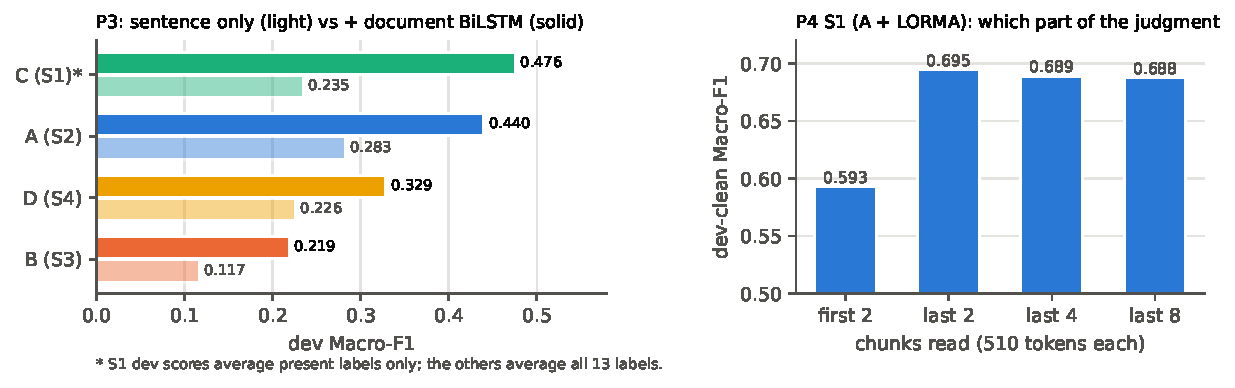
\includegraphics[width=0.78\textwidth]{fig4_context_and_sections.pdf}
\caption{Left: Phase-3 document context (sentence-only probe vs document BiLSTM). Right: Phase-4 section analysis for \A{}+LORMA. \C's 0.476 averages only the labels that appear in dev; the others average all 13 labels.}\label{fig:context}
\end{figure}
\begin{figure}[h]\centering
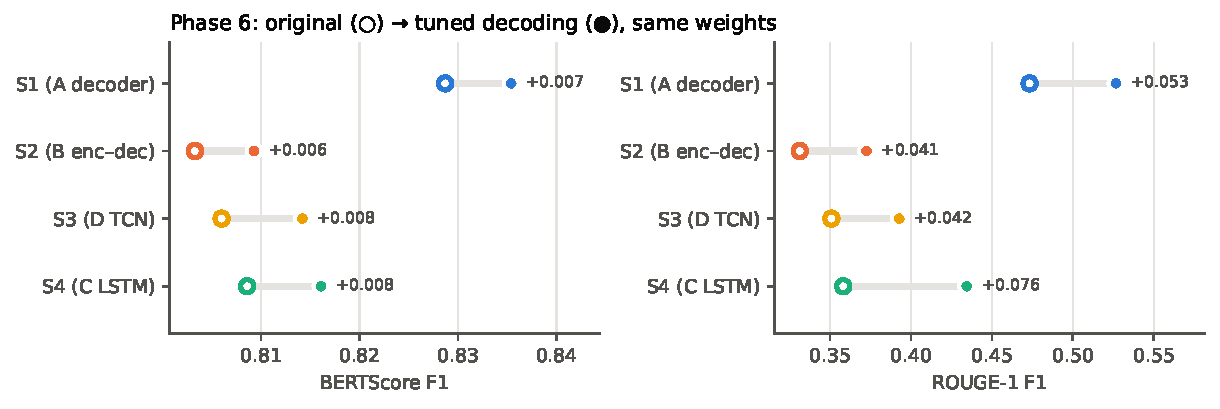
\includegraphics[width=0.75\textwidth]{fig3_phase6_decoding_tuning.pdf}
\caption{Phase 6: the same weights with the original vs the tuned decoding, for all four models.}\label{fig:dec}
\end{figure}

\paragraph{Phase-7 KD report} (100 dev documents, first 4 + last 4 chunks, one T4).
\begin{itemize}
\item \textbf{Teacher:} 126.7M parameters, 7.04\,s to encode, dev 0.269, test 0.2534.
\item \textbf{Student:} 83.6M parameters, 3.54\,s, dev 0.280, test 0.2374.
\item \textbf{Comparison:} top-7 agreement with the teacher was 49\%. The teacher rebuilt from its checkpoint reproduces the saved vectors (cosine 1.000).
\end{itemize}

\paragraph{Phase-7 error pattern.}
\begin{itemize}
\item Queries with one relevant case reach precision@7 of only 0.05--0.08.
\item Queries with 16 or more relevant cases reach precision 0.38--0.56, but recall only 0.09--0.13.
\item S1 found no relevant case for 18 of 118 dev queries.
\end{itemize}

\paragraph{Per-phase details.} Each \texttt{code/phaseN/README.md} has the full data analysis, per-class results, error examples and Kaggle links for its phase. The experiment log in \texttt{docs/} records every run in order.
\end{document}
